\documentclass[pdf]{beamer}
\usetheme{Darmstadt}
\mode<presentation>{}

% Use the postscript times font!
\usepackage{fancyvrb}
\usepackage{times}
\usepackage{soul}
\usepackage{url}
\usepackage[utf8]{inputenc}
\usepackage[small]{caption}
\usepackage{graphicx}
\usepackage{amsmath}
\usepackage{booktabs}
\usepackage{algorithm}
\usepackage{multicol}
\usepackage{algorithmic}
\usepackage{wrapfig}
\urlstyle{same}

\newcommand{\?}{\ensuremath{^\texttt{\bf [CITATION~NEEDED]}}}
% the following package is optional:
%\usepackage{latexsym} 

\title{Deep Text Prior: Weakly Supervised Learning for Assertion Classification}
% If the paper title is too long for the running head, you can set
% an abbreviated paper title here
%
\author{Vadim Liventsev\inst{1,2,3} \and
Irina Fedulova\inst{1} \and
Dmitry Dylov\inst{2}}
%
\institute{
\inst{1} Work done at Philips Innovation Labs RUS \\
\{Vadim.Liventsev,Irina.Fedulova\}@philips.com \and
\inst{2} Work done at Skolkovo Institure of Science and Technology \\
\{Vadim.Liventsev,D.Dylov\}@skoltech.ru \and
\inst{3} Currently at Eindhoven University of Technology \\
v.liventsev@tue.nl
}
\begin{document}

\begin{frame}
\titlepage
\end{frame}

\section{Introduction}
\label{sec:intro}

\subsection{Problem statement}

\begin{frame}{Pop quiz}

\begin{center}
\textbf{INDICATION:} Evaluate for \emph{pneumonia}
\end{center}

\pause

\begin{enumerate}[A.]
\item This patient has \emph{pneumonia}
\item This patient does not have \emph{pneumonia}
\item \alert<2>{We don't know}
\end{enumerate}

\end{frame}

\begin{frame}{Pop quiz}

\begin{center}
\textbf{IMPRESSION:} No evidence of \emph{pneumonia}
\end{center}

\begin{enumerate}[A.]
\item This patient has \emph{pneumonia}
\item \alert<2>{This patient does not have \emph{pneumonia}}
\item We don't know
\end{enumerate}

\end{frame}

\begin{frame}{Pop quiz}
\begin{center}
\textbf{FINDINGS:} Developing \emph{pneumonia} should be excluded by repeat image.
\end{center}

\begin{enumerate}[A.]
\item This patient has \emph{pneumonia}
\item This patient does not have \emph{pneumonia}
\item \alert<2>{We don't know}
\end{enumerate}

\end{frame}

\begin{frame}{Pop quiz}
\begin{center}
\textbf{IMPRESSION:} Effusions represent area of atelectasis, although \emph{pneumonia} could	also have this appearance.
\end{center}

\begin{enumerate}[A.]
\item This patient has \emph{pneumonia}
\item This patient does not have \emph{pneumonia}
\item \alert<2>{We don't know}
\end{enumerate}

\end{frame}

\begin{frame}{Assertion classification problem}

Features:

\begin{equation}
\underset{\text{metadata}}{\text{INDICATION}}: \text{Evaluate for} \underset{\text{concept of interest}}{\text{pneumonia}}
\end{equation}

\pause

Classes:

\begin{description}
\item[positive] the author states that the patient \emph{has} the condition
\item[negative] the author asserts that the patient does \emph{not} have the condition
\item[speculative] the author mentions the condition, but \emph{does not assert anything} as to whether the patient has it
\end{description}

\end{frame}

\subsection{Motivation}

\begin{frame}{Landscape of Artificial Intelligence in Medicine}

\begin{figure}
\centering
\makebox[\linewidth][c]{
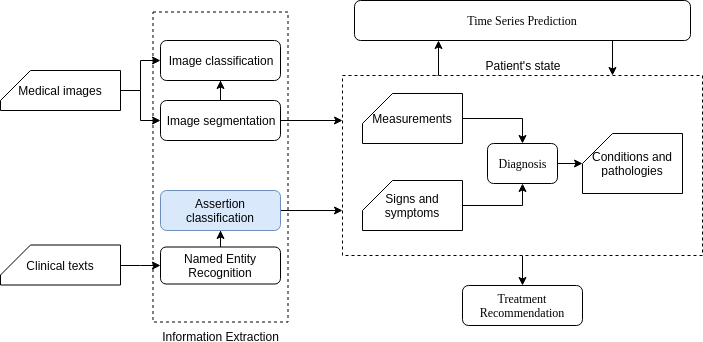
\includegraphics[width=\textwidth]{img/medical-tasks.png}
}
\caption{Medical AI task graph}
\label{fig_task_graph}
\end{figure}

\end{frame}

\begin{frame}{Landscape of Artificial Intelligence in Medicine}

\begin{figure}
\centering
\makebox[\linewidth][c]{
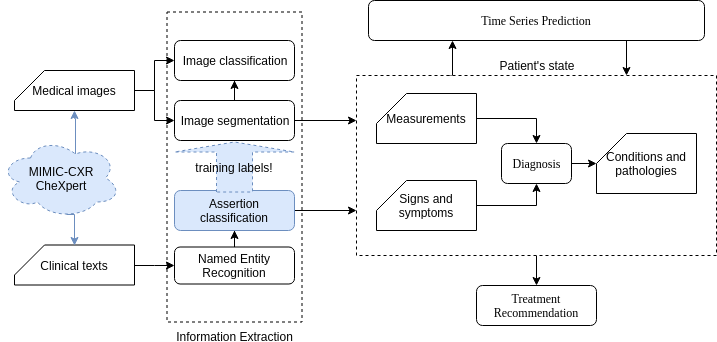
\includegraphics[width=\textwidth]{img/medical-tasks-point.png}
}
\caption{Medical AI task graph}
\label{fig_task_graph_point}
\end{figure}

\end{frame}

\begin{frame}[fragile]{Datasets}

\begin{figure}
\begin{center}
\tiny
\begin{BVerbatim}

[**Hospital 9**] MEDICAL CONDITION:
  64 year old immunocompromised women with persistent cough/SOB and fluid 
  overload
 REASON FOR THIS EXAMINATION:
  ?pna, pleural effusions                                                         
 ______________________________________________________________________________
                                 FINAL REPORT
 CHEST RADIOGRAPH
 
 INDICATION:  Immunocompromised woman, shortness of breath.
 
 COMPARISON:  [**2192-12-8**].
 
 FINDINGS:  As compared to the previous radiograph, there is no relevant
 change.  The lung volumes have increased.  The monitoring and support devices
 are all unchanged.  Unchanged scarring at the left and right lung bases but no
 newly appeared parenchymal opacity.  Unchanged size of the cardiac silhouette.

\end{BVerbatim}
\end{center}
\caption{A sample radiology report from MIMIC-CXR}
\label{mimic-report}
\end{figure}

\end{frame}

\begin{frame}{Datasets}

\begin{figure}
\centering
\makebox[\linewidth][c]{
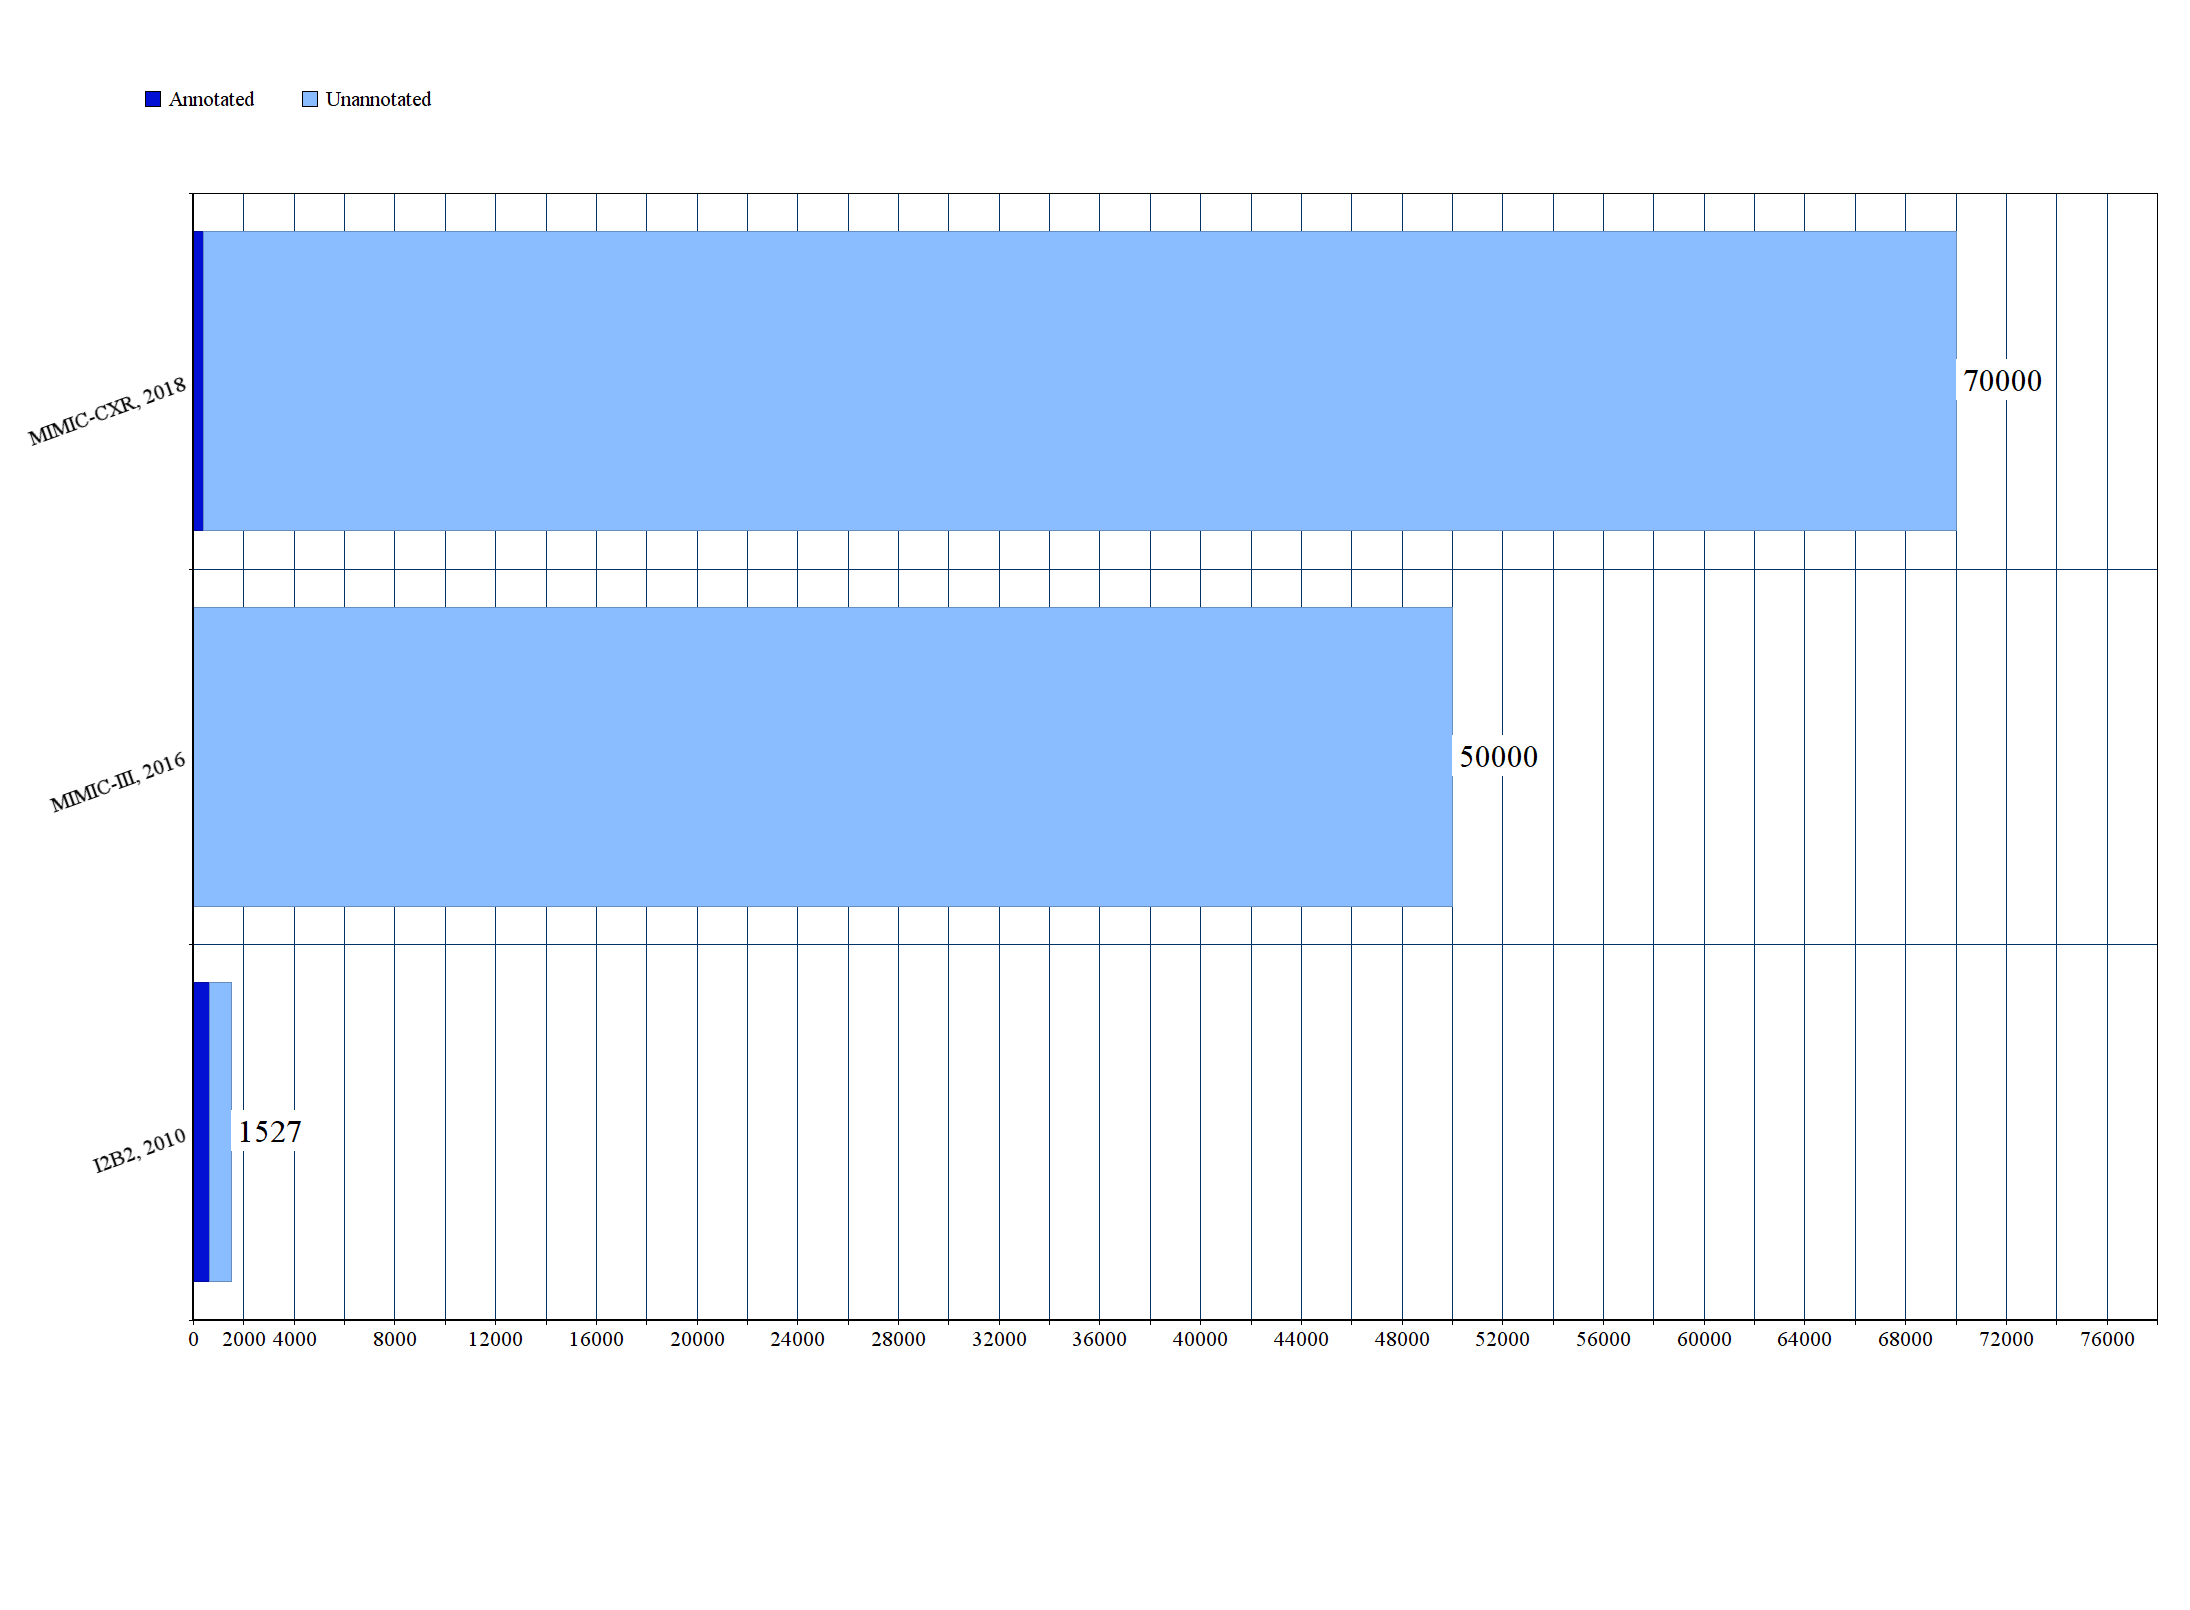
\includegraphics[width=\textwidth]{img/ann.png}
}
\caption{Assertion annotations in clinical text datasets}
\label{fig_datasets}
\end{figure}

\end{frame}

\section{Related work}

\begin{frame}[fragile]{Rule-based approaches}

\begin{figure}
\begin{center}
\tiny
\begin{BVerbatim}
{} <{dependency:/nmod:of|nmod:for/} ({lemma:/evidence/} >{dependency:/neg/} {})
\end{BVerbatim}
\end{center}
\caption{A sample negation cue from NegBio. Detects the phrase "No evidence of/for X"}
\end{figure}

Typical pipeline:

\begin{enumerate}
\item Part of speech tagging
\item Dependency parsing
\item Complicated feature extraction
\item Negation and speculation cues
\end{enumerate}

\pause

Issues:

\begin{itemize}
\item Generalisation issues
\item Language bias
\item Dataset bias
\end{itemize}

% Parse tree?

\end{frame}

\begin{frame}{Statistical approaches}
\label{sec:statistical}

Typical pipeline:

\begin{enumerate}
\item Part of speech tagging
\item Dependency parsing
\item Complicated feature extraction
\item Support Vector Machines
\end{enumerate}

\pause

Issues:

\begin{itemize}
\item Generalisation issues
\item Language bias
\item Dataset bias
\end{itemize}
\end{frame}

\section{Methodology}

\begin{frame}{Our approach}

Incorporate as much prior knowledge as possible into our models:

\begin{itemize}
\item Incorporate metadata into assertion specification
\item Use state of the art pretrained language models (ELMo) for sentence representation
\item Use prototype network approach to incorporate relationships between classes
\item Use specialized model architectures for the task at hand
\item Use heuristic algorithms to pretrain the models with inexact supervision
\end{itemize}

\end{frame}

\begin{frame}{Assertion representation}

\begin{figure}
\centering
\makebox[\linewidth][c]{
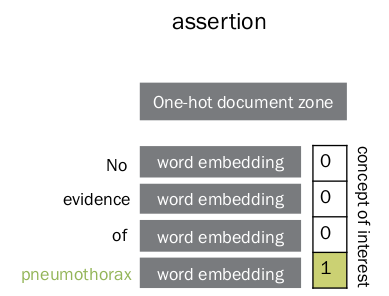
\includegraphics[width=0.5\textwidth]{img/ass.png}
}
\caption{Vector representation of an assertion}
\label{fig_assertion}
\end{figure}

\end{frame}

\begin{frame}{Prototype networks}

\begin{equation}
\text{CMSE}(\text{TC}, \text{PC}, \text{TR}, \text{PR}) = (\text{TC} - \text{PC})^2 + \text{TC} * (\text{TR} - \text{PR})^2
\end{equation}

\begin{columns}[t]

\begin{column}{5cm}

\begin{description}
\item[T] true
\item[P] predicted
\item[R] reality
\item[C] confidence
\end{description}

\end{column}

\begin{column}{5cm}
\begin{figure}
\centering
\makebox[\linewidth][c]{
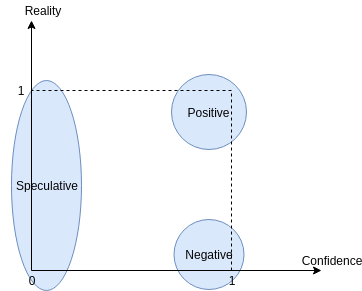
\includegraphics[width=\textwidth]{img/prototype.png}
}
\caption{Class prototypes in reality-confidence space}
\label{fig_prototype}
\end{figure}
\end{column}

\end{columns}

\end{frame}

\begin{frame}{Models}

\begin{figure}
\centering
\makebox[\linewidth][c]{
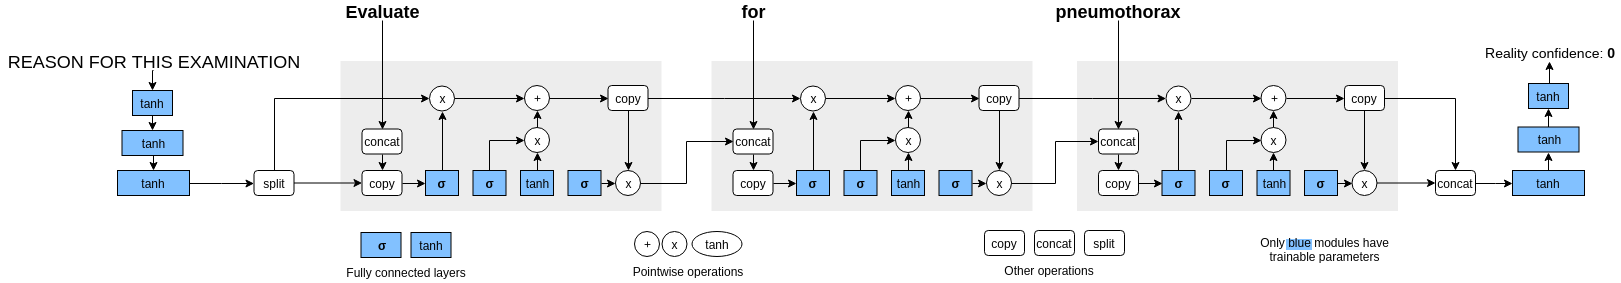
\includegraphics[width=\textwidth]{img/lstm.png}
}
\caption{LSTM model}
\label{fig_lstm}
\end{figure}

\end{frame}

\begin{frame}{Models}

\begin{figure}
\centering
\makebox[\linewidth][c]{
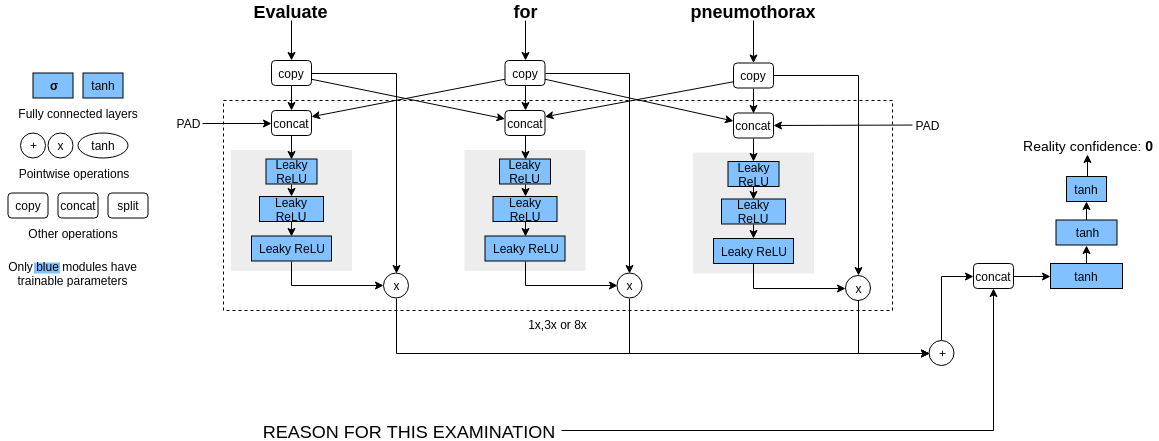
\includegraphics[width=\textwidth]{img/attention.png}
}
\caption{Attention-based model}
\label{fig_attention}
\end{figure}

\end{frame}

\begin{frame}{NegBio+ heuristic algorithm}

\begin{description}
\item[speculative] if the assertion is in INDICATION, REASON FOR THIS EXAMINATION or similar section
\item[negative] if one of NegBio negation cues fires ("no X", "no evidence of X")
\item[positive] otherwise
\end{description}

\end{frame}

\begin{frame}{Weakly supervised learning schedules}

\begin{enumerate}
\item \emph{Classic}. Initialize weights randomly, then $\underset{\text{weights}}{\text{minimize}} ||\text{model}_{\text{weights}}(X) - y_{\text{true}}||$
\item \emph{Deep Prior}. Initialize weights randomly, $\underset{\text{weights}}{\text{minimize}} ||\text{model}_{\text{weights}}(X) - \text{NegBio+}(X)||$.
\item \emph{Transfer}. Use the weights obtained with \emph{Deep Prior} as initialization, $\underset{\text{weights}}{\text{minimize}} ||\text{model}_{\text{weights}}(X) - y_{\text{true}}||$.
\end{enumerate}

\end{frame}

\section{Results}
\label{sec:results}

\begin{frame}{Cross-validation results}

\begin{table}
\caption{Accuracy on I2B2 Challenge}
\label{i2b2-accuracy}
\begin{tabular}{llrrr}
\toprule
 & ctakes & 0.796  & 0.796 & 0.796  \\
\midrule
Vectors &      Model         &  Classic &  Deep Prior &  Transfer \\
\midrule
                   elmo &          attention1 &    0.625 &       0.704 &     0.756 \\
                   elmo &          attention8 &    0.621 &       0.706 &     0.738 \\
                   elmo &            lstm1024 &    0.798 &       0.755 &     0.866 \\
                   elmo &             lstm128 &    0.846 &       0.747 &     0.868 \\
                   elmo &             lstm512 &    \textbf{0.858} &       0.733 &     \textbf{0.858} \\
                   elmo &               lstm8 &    0.621 &       0.624 &     0.673 \\
\bottomrule
\end{tabular}
\end{table}

\end{frame}

\begin{frame}{Cross-validation results}

\begin{table}
\caption{Accuracy on MIMIC-CXR-FREQ}
\label{mimic-freq-accuracy}
\small
\begin{tabular}{llrrr}
\toprule
 & NegBio+ & 0.834  & 0.834 & 0.834  \\
\midrule
Vectors &       Model        &  Classic &  Deep Prior &  Transfer \\
\midrule
                   elmo &        attention1 &    0.615 &       0.803 &    0.932 \\
                   elmo &        attention3 &    0.863 &       0.225 &    0.950 \\
                   elmo &        attention8 &    0.919 &       0.576 &    0.944 \\
                   elmo &             lstm8 &    0.639 &       0.878 &    0.898 \\
                   elmo &           lstm128 &    0.927 &       0.873 &    0.967 \\
                   elmo &           lstm512 &    0.912 &       0.873 &    \textbf{0.975} \\
                   elmo &          lstm1024 &    0.785 &       0.876 &    0.939 \\
               fasttext &        attention1 &    0.610 &       0.429 &    0.870 \\
               fasttext &        attention3 &    0.944 &       0.325 &    0.773 \\
               fasttext &        attention8 &    0.778 &       0.441 &    0.838 \\
               fasttext &             lstm8 &    0.276 &       0.388 &    0.058 \\
               fasttext &           lstm128 &    0.705 &       0.914 &    0.929 \\
               fasttext &           lstm512 &    0.748 &       0.381 &    0.841 \\
               fasttext &          lstm1024 &    0.578 &       0.309 &    0.796 \\
\bottomrule
\end{tabular}
\end{table}

\end{frame}

\begin{frame}{Cross-validation results}

\begin{table}
\caption{Accuracy on MIMIC-CXR-LONG}
\label{mimic-long-accuracy}
\begin{tabular}{llrrr}
\toprule
 & NegBio+ & 0.71  & 0.71 & 0.71  \\
\midrule
Vectors &        Model       &  Classic &  Deep Prior &  Transfer \\
\midrule
                   elmo &  attention3 &    0.800 &       0.770 &     0.683 \\
                   elmo &  attention8 &    0.833 &       0.710 &     \textbf{0.843} \\
                   elmo &     lstm128 &    0.716 &       0.690 &     0.750 \\
                   elmo &     lstm512 &    0.763 &       0.710 &     0.691 \\
                   elmo &       lstm8 &    0.721 &       0.700 &     0.821 \\
               fasttext &  attention3 &    0.722 &       0.680 &     0.821 \\
               fasttext &  attention8 &    0.810 &       0.750 &     0.739 \\
               fasttext &     lstm128 &    0.686 &       0.690 &     0.722 \\
               fasttext &     lstm512 &    0.862 &       0.700 &     0.788 \\
               fasttext &       lstm8 &    0.830 &       0.690 &     0.694 \\
\bottomrule
\end{tabular}
\end{table}

\end{frame}

\begin{frame}{Result highlights}

\begin{table}
\caption{Heuristic pretraining effect on MIMIC-CXR-FREQ}
\label{pretraining-effect}
\begin{tabular}{llrr}
\toprule
Vectors &       Model        &  Classic &  Transfer \\
\midrule
                   elmo &        attention1 &    0.615 &    + 0.317 \\
                   elmo &        attention3 &    0.863 &    + 0.097 \\
                   elmo &        attention8 &    0.919 &    + 0.025 \\
                   elmo &             lstm8 &    0.639 &    + 0.249 \\
                   elmo &           lstm128 &    0.927 &    + 0.040 \\
                   elmo &           lstm512 &    0.912 &    + 0.063 \\
                   elmo &          lstm1024 &    0.785 &    + 0.154 \\
               fasttext &        attention1 &    0.610 &    + 0.260 \\
               fasttext &        attention8 &    0.778 &    + 0.050 \\
               fasttext &           lstm512 &    0.748 &    + 0.097 \\
               fasttext &          lstm1024 &    0.578 &    + 0.218 \\
\bottomrule
\end{tabular}
\end{table}

\end{frame}

\begin{frame}{Result highlights}

\begin{table}
\caption{Contextualized embeddings effect on MIMIC-CXR-FREQ}
\label{context-effect}
\small
\begin{tabular}{llrr}
\toprule
 Model       &  Schedule & fasttext &  elmo \\
\midrule
lstm8 & Classic & 0.276 & + 0.363 \\
lstm8 & Deep Prior & 0.388 & + 0.490 \\
lstm8 & Transfer & 0.058 & + 0.848 \\
lstm512 & Classic & 0.748 & + 0.164 \\
lstm512 & Deep Prior & 0.381 & + 0.492 \\
lstm512 & Transfer & 0.841 & + 0.134 \\
lstm1024 & Classic & 0.578 & + 0.207 \\
lstm1024 & Deep Prior & 0.309 & + 0.567 \\
lstm1024 & Transfer & 0.796 & + 0.143 \\
attention1 & Classic & 0.610 & + 0.164 \\
attention1 & Deep Prior & 0.429 & + 0.374 \\
attention1 & Transfer & 0.870 & + 0.062 \\
\bottomrule
\end{tabular}
\end{table}

\end{frame}

\begin{frame}{Result highlights}

\begin{table}
\caption{Deep prior effect on MIMIC-CXR-FREQ}
\label{deepprior-effect}
\begin{tabular}{llr}
\toprule
 Vectors & Model       &  Advantage over NegBio+ \\
\midrule
                   elmo &             lstm8 &    + 0.044 \\
                   elmo &           lstm128 &    + 0.039 \\
                   elmo &           lstm512 &    + 0.039 \\
                   elmo &          lstm1024 &   + 0.042 \\
\bottomrule
\end{tabular}
\end{table}

\end{frame}

\section{Discussion}

\begin{frame}{Neural relaxation of algorithms}

Given $X$ and $heuristic(X)$ one can outperform $heuristic(X)$ by solving

\begin{equation}
\underset{\text{weights}}{\text{minimize}} ||\text{model}_{\text{weights}}(X) - \text{heuristic}(X)||
\end{equation} 

\pause

\alert{Neural networks are priors!}

On a different problem (mild/moderate/severe classification) we managed to achieve +30\% improvement via this method

\end{frame}

\begin{frame}{\st{Commercial break} Acknowledgments} 

\begin{columns}[T]

\begin{column}{5cm}

Organizations:


\includegraphics[width=0.5\textwidth]{img/skoltech.png}

\includegraphics[width=0.5\textwidth]{img/philips.png}

People:

Artem Shelmanov, Ilya Sochenkov, Francis Tyers

\end{column}

\begin{column}{5cm}
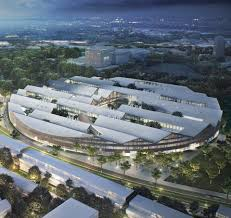
\includegraphics[width=\textwidth]{img/skoltech-campus.jpeg}
\end{column}

\end{columns}


\end{frame}

\begin{frame}{Ask us anything}

Vadim.Liventsev@skoltech.ru \\
v.liventsev@tue.nl \\
Irina.Fedulova@philips.com \\
D.Dylov@skoltech.ru

\end{frame}

\end{document}